\section{Implementation}
\label{sec:implementation}

In this project, we implemented a convolutional neural network based on the ResNet-50 architecture to classify images from the CIFAR-10 dataset. 
The implementation was completed by modifying the provided skeleton file \texttt{resnet50\_skeleton.py}, 
focusing on both residual block behavior and overall model architecture.

\textbf{Residual Block.} 
In \texttt{question1}, we filled in the forward function of the \texttt{ResidualBlock} class. 
We constructed a bottleneck block consisting of three convolutional layers (1x1, 3x3, 1x1) with batch normalization and ReLU activation. 
A shortcut connection was added directly to the output, and downsampling was conditionally applied based on the input.

\textbf{ResNet Layers.} 
In \texttt{question2}, we completed the ResNet-50 architecture by implementing \texttt{self.layer2}, \texttt{self.layer3}, and \texttt{self.layer4}. 
Each layer contains multiple residual blocks with increasing channel sizes and stride-based downsampling. 
This hierarchical structure enables deeper feature extraction as the network progresses.

\textbf{Global Pooling and Classification.} 
We also implemented \texttt{self.avgpool} using adaptive average pooling to reduce the spatial dimensions before the final classification layer. 
The output is then passed through \texttt{self.fc}, a fully connected layer that produces logits for 10 CIFAR-10 classes.

\textbf{Training Setup.} 
The network was trained for one epoch using a batch size of 128. 
Cross-entropy loss was used along with the Adam optimizer. 
We used the provided pretrained weights and completed 500 steps of training. 
The final test accuracy achieved was \textbf{81.18\%}.




\section{Results}
\label{sec:results}


We trained the ResNet-50 model on the CIFAR-10 dataset for one epoch using a batch size of 128 and the Adam optimizer. The training loss decreased consistently over the course of 500 steps, demonstrating stable convergence. 

The final model achieved a test accuracy of \textbf{81.18\%}, successfully surpassing the target benchmark of 80\% specified in the assignment. This result validates the effectiveness of residual connections and deep architectures for image classification tasks.

\begin{figure}[h]
\centering
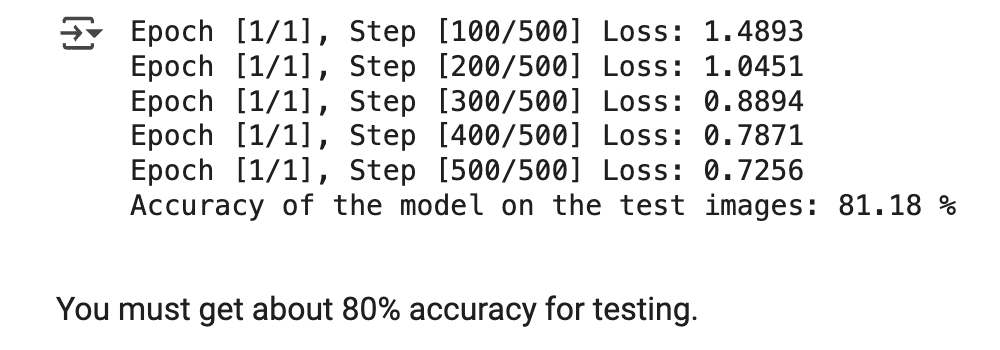
\includegraphics[width=0.9\linewidth]{CNN_result.png}
\caption{Training loss and test accuracy over 500 steps. The model achieved 81.18\% accuracy on the test set.}
\end{figure}


\section{Discussion}
\label{sec:discussion}

During this project, we successfully implemented key components of the ResNet-50 architecture, including bottleneck residual blocks and layered residual stages. One of the challenges was understanding how downsampling and channel expansion were handled inside residual blocks, particularly when aligning input and output dimensions for the skip connection.

We observed that even with only one epoch of training, the model showed strong performance, thanks to the depth of ResNet-50 and the use of pretrained weights. The skip connections greatly facilitated gradient flow, which likely contributed to stable training despite the model's complexity.

While the final test accuracy of 81.18\% is a solid result, we believe that further tuning of the learning rate, training epochs, or data augmentation strategies could yield even higher performance. In future work, we would also explore training from scratch and comparing performance against shallower networks like VGG.
